\documentclass[aima331_lecturenotes_ku.tex]{subfiles}

\begin{document}
\chapter{Vector Calculus}
\section{Basics}
\begin{mdframed}
  scalars, vectors, their notations, length of a vector, norm of a vector, unit vector, angle between two vectors, inner product, orthogonal vectors, orthonormal vectors,
\end{mdframed}
Physically, a vector is a quantity having both magnitude and direction. Mathematically, a vector is an element of a vector space. A vector is a compound mathematical object constructed from simpler objects called scalars.

\begin{itemize}
\item \textbf{Equality of Vectors} \\[1mm]
  Two vectors $a$ and $b$ are said to be equal if they have same length and same direction. Hence a vector can be arbitrarily translated; i.e, its initial point can be chosen arbitrarily.

\item \textbf{Plane Vectors and Space Vectors} \\[1mm]
  The vectors of the vector space $\mathbb{R}^2$ are called plane vectors and the vectors of the vector space $\mathbb{R}^3$ are called space vectors. Plane vectors are $2-D$ vectors and space vectors are $3-D$ vectors.

  \begin{figure}[h]
    \centering
    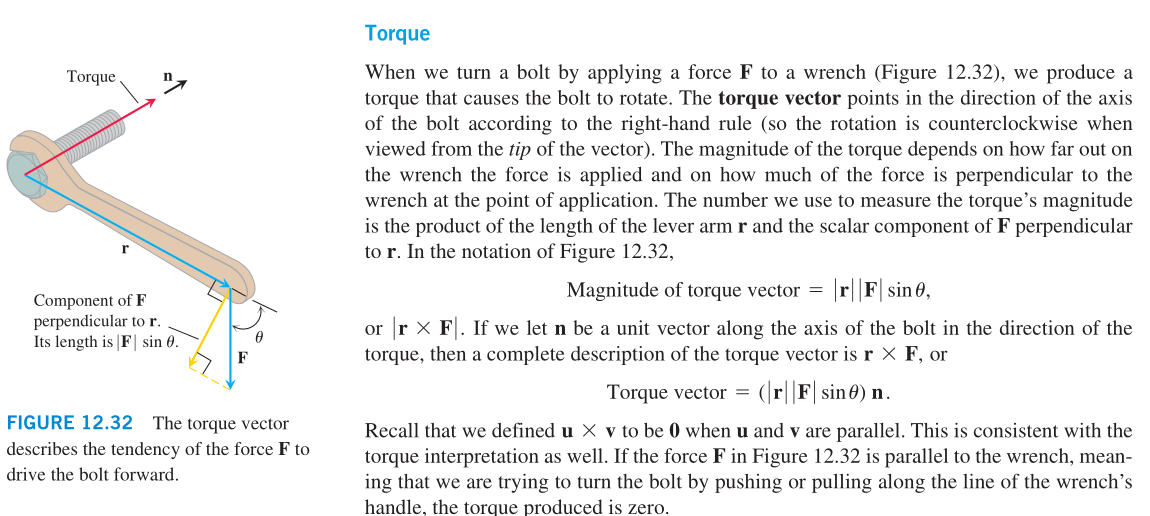
\includegraphics[width=15cm, height=8cm]{torque.png}
  \end{figure}

\item \textbf{Vector Product} \\[1mm]
  Let $a=(a_1, a_2, a_3)$ and $b=(b_1, b_2, b_3)$ be two space vectors. Then, their vector product is denoted by $a \times b$ and defined as a new vector such that \\
  $a \times b = (a_2b_3 - b_2a_3, a_3b_1 - b_3a_1, a_1b_2-b_1a_2)$

\item \textbf{Right Handed Coordinate System} \\[1mm]
  Here the coordinate system is right-handed, meaning the unit vectors $\hat{i}, \;\;\; \hat{j}, \;\;\; \hat{k}$ forms a right-handed triple.
  \textit{What is a right-handed triple?}
\end{itemize}
\section{Vector Calculus}
\subsection{Scalar Functions and Vector Functions}
\begin{itemize}
\item A function whose co-domain is a scalar set is called a scalar function. For example, $f: \mathbb{R}^2 \to \mathbb{R}$ defined by $f(x,y)=x$ is a \textbf{scalar function}. We say that a scalar function defines a scalar field in that domain. Examples of scalar fields are the temperature field in a body or the pressure field of the air in the earth's atmosphere.

\item A function whose co-domain is a vector space is called a \textbf{vector function}. For example, $f: \mathbb{R}^2 \to \mathbb{R}^2$ defined by $v(x,y)=(y,x)$ is a vector function. Moreover, a vector function on $D$ is a rule that assigns a vector to each element in $D$. The common vector functions are the plane vector functions and the space vector functions.

\item So, the mathematics of a vector function is a mathematics of a multivariable function and the vector calculus is \textbf{multivariable calculus}.

\item A \textbf{vector field} is a field that is defined by a vector function. For example magnetic field of a bar magnet is a vector field, velocity field of a rotating disc is a vector field, they are characterized by the vector functions, force and velocity. Another vector field is the earth's gravitational field. This one is a three dimensional vector field. \textit{Try drawing these fields in your copy}.
\end{itemize}

\subsection{Vector Field}
Mathematically, a vector field is a field that is defined by a vector function.
\begin{itemize}
\item Suppose a region in the plane or in space is occupied by a moving fluid, such as water. The fluid is made up of a large number of particles, and at any instant of time, a particle has a velocity $\vec{v}$. At different points of the region at a given time, these velocities can vary. We can think of a velocity vector being attached to each point of the fluid representing the velocity of a particle at that point. Such a fluid flow is an example of a vector field.

\item The tangent $T$ for a curve and normal vectors $N$ for a surface in a space both form vector fields along the curve.

\item The gradient of a scalar function in a space we obtain a three-dimensional field on the surface.
  \begin{figure}[h]
     \label{streamline}
\centering
\begin{subfigure}{0.32\textwidth}
  \label{streamline}
  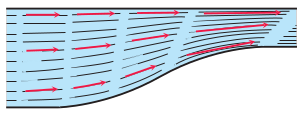
\includegraphics[height=4cm, width=\textwidth]{streamline.png}
  \caption{velocity field of a stream line flow}
\end{subfigure}
\hfill
\begin{subfigure}{0.31\textwidth}
  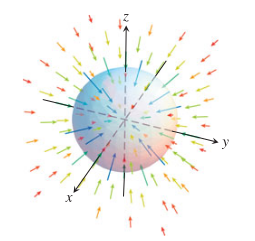
\includegraphics[height=6cm, width=\textwidth]{gravitational.png}
  \caption{gravitational field}
\end{subfigure}
\hfill
\begin{subfigure}{0.32\textwidth}
  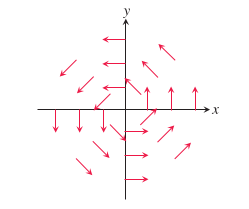
\includegraphics[height=6cm, width=\textwidth]{radial.png}
  \caption{spin field of a rotating vectors}
\end{subfigure}
\end{figure}
\end{itemize}

\begin{figure}[h]
  \centering
  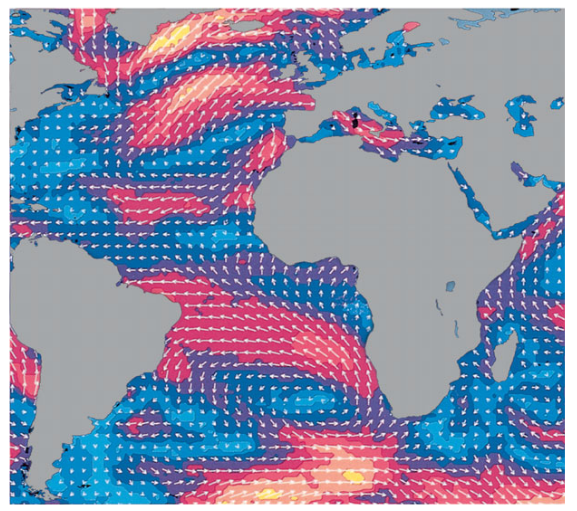
\includegraphics[height=7cm, width=12cm]{weather.png}
  \caption{Wind measurement over world's oceans.}
  \label{weather}
\end{figure}


\subsection{Curves in Space}
When a particle moves through space during a time interval $I$, we think of the particle's coordinates as functions defined on $I$:
\begin{equation}
  \label{coordinate}
  x=f(t), \hspace{5mm} y=g(t), \hspace{5mm} z=h(t), \hspace{5mm} t \in I
\end{equation}
The points $(x,y,z)=(f(t),g(t),h(t)), \;\; t \in I$ make up the curve in space that we call the particle's path. The equation~\ref{coordinate} parametrize the curve. A curve in space can also be represented in vector form. The vector
\begin{equation}
  \label{vector}
  r(t) = \vec{OP} = f(t)\hat{i} + g(t)\hat{j} + h(t)\hat{k}
\end{equation}
The equation~\ref{vector} defines a \textbf{vector valued function} or a vector function. The circle $x^2 + y^2 = 1$ is a scalar function whereas, the same circle $(x,y) = (cost, sint)$ is a vector function.
A major application of vector calculus concerns curves and surfaces and their use in physics and geometry. This field is called \textbf{differential geometry}. It plays a role in mechanics, computer-aided and traditional engineering design, geodesy and geography, space travel, and relativity theory.\\
Curves in space may occur as paths of moving bodies. This and other applications motivate \textit{parametric representations} with parameter $t$, which may be time or something else: $r(t)=(x(t), \; y(t), \; z(t)) = x(t)\hat{i} + y(t)\hat{k} + z(t)\hat{k}$. To each value of $t$ there corresponds a point of $C$ with position vector $r(t)$. Moreover, the sense of increasing $t$, called the positive sense on the curve, induces an \textbf{orientation} of the curve, a direction of travel along the curve. The sense of decreasing $t$ is then called the negative sense on the curve.
\begin{wrapfigure}{r}{0.24\textwidth}
  \centering
  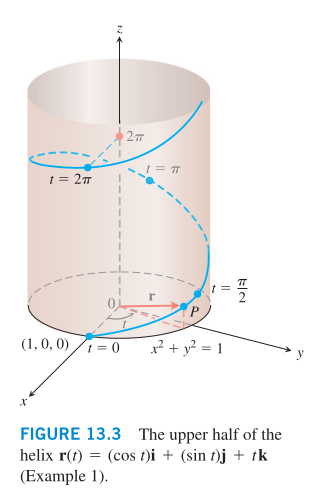
\includegraphics[width=0.3\textwidth]{helix.png}
  \label{fig:img1}
\end{wrapfigure}

\begin{example}
  The ellipse in the $xy$-plane with center at the origin is $$\frac{x^2}{a^2} + \frac{y^2}{b^2}  = 1, \;\;\;\; z=0$$. The corresponding vector function with the parameter $t$ is $$r(t) = (acost, \; bsint, 0)= acost \;\hat{i} + bsint \;\hat{j}$$
  \begin{itemize}
  \item Similarly the parametric equation of a \textbf{straight line} is $r(t) = \vec{a} + t\vec{b}$.
  \item The parametric equation of \textbf{circular helix} that lies on the cylinder $x^2+y^2=a^2$ is $r(t)=(acost, \; asint, \;ct)$. If $c>0$ the helix is shaped like a right-handed screw, else it looks like a left-handed screw. What happens if $c=0$?
  \end{itemize}
\end{example}
\subsection{Exercise}
\begin{enumerate}
\item Write a parametric equation of a general plane.
\item Find a parametric equation of the following:
  \begin{multicols}{2}
    a). Circle of radius 3, center $(4,6)$.
    \columnbreak

    b). Parabola $y=4x^2$
  \end{multicols}

\item What curves are represented by the following?
  \begin{multicols}{3}
    a). $(2+cos3t, -2+sin3t, 5)$
    \columnbreak


    b). $(t, 1/t, 0)$
    \columnbreak

    c). $(cosht, \;sinht, \;0)$
  \end{multicols}
\item Show that setting $t=-t$ reverses the orientation of $(acost, \; asint, \; 0)$.
\end{enumerate}

\subsection{Derivative of a Vector function}
When a vector-valued function changes, the change can occur in both magnitude and direction, so the derivative is itself a vector. The integral of a vector valued function is also a vector. We use the calculus of these functions to describe the paths and motions of objects moving in plane or in a space.
\begin{mdframed}
  The vector function $r(t) = f(t)\hat{i} + g(t)\hat{j} + h(t)\hat{k}$ has a derivative at $t$ if $f,g,$ and $h$ have derivatives at $t$. The derivative is the vector function
  $$r'(t) = \frac{dr}{dt} = \lim_{\Delta t \to 0}\;\; \frac{r(t+\Delta t) - r(t)}{\Delta t} = \frac{df}{dt}\hat{i} + \frac{dg}{dt}\hat{j} + \frac{dh}{dt}\hat{k}$$
\end{mdframed}
The vector $r'(t)$, when different from $0$, is defined to be the vector \textbf{tangent} to the curve at $t$. The \textbf{tangent line} to the curve at a point defined by $t_0$ is defined to be the line through the point parallel to $r'(t_0)$. We require $r'(t) \neq 0 $ for a \textbf{smooth} curve to make sure the curve has a continuously turning tangent at each point. On a smooth curve, there are no sharp corners or cusps.
\begin{figure}[h]
  \centering
  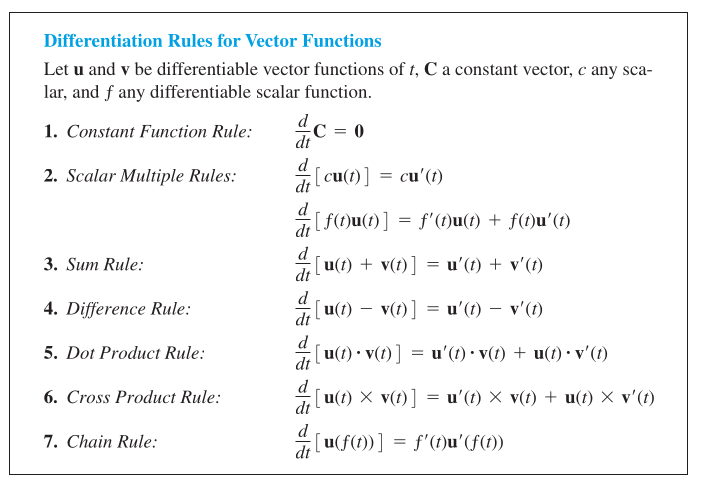
\includegraphics[width=11cm, height=8cm]{diff_rule.png}
\end{figure}
\subsection{Exercise}
\begin{enumerate}
\item Explain geometrically, how $r'(t)$ is a vector along the tangent to the curve $r$ at $t$.

\item   Find the velocity, speed and acceleration of a particle that is moving along the curve $r(t) = 2 cost\hat{i} + 2sint \hat{j} + cos^2t \hat{k}$ in time $t$.
\item Explain the derivative of a vector function of constant length.\textit{(Take the help of dot product.)}
\item What kind of surfaces are the level surfaces $f(x,y,z)=const$?
  \begin{multicols}{3}
    a). $f=x^2+y^2+4z^2$
    \columnbreak

    b). $f=z-\sqrt{x^2-y^2}$
    \columnbreak

    c). $f=4x+3y-5z$
  \end{multicols}
\item Sketch the vector fields of:
  \begin{multicols}{3}
    a). $v=i-j$
    \columnbreak

    b). $v=yi+xj$
    \columnbreak

    c). $v=(x-y)i + (x+y)j$
  \end{multicols}

\item Find the first and second derivative of: $[4cost,\; 4sint, \; 2t]$
\item Find the first partial derivatives of: $[e^xcosy,\; e^xsiny]$
\end{enumerate}

\section{Multivariable Calculus Review}
Many functions depend on more than one independent variable. For instance, the volume of a right circular cylinder is a function \(V=\pi r^2 h\) of its radius and height, so it a function \(V(r,h)\) of two variables \(r\) and \(h\). Real-valued functions of several independent real variables  are defined analogously to functions in the single-variable case.

\begin{mdframed}
  \begin{definition}
    Suppose \(D\) is a set of \(n-tuples\) of real numbers \((x_1,x_2,...,x_n)\). A \textbf{real-valued function} \(f\) on \(D\) is a rule that assigns a unique (single) real number \[w=f(x_1,x_2,...,x_n)\] to each element of \(D\). The set \(D\) is the function's \textbf{domain}, and \(f\) is said to be a function of \(n\) \textbf{independent variables} \(x_1\) to \(x_2\).
  \end{definition}
\end{mdframed}
If \(f\) is a function of two independent variables, we usually call the independent variables \(x\) and \(y\) and the dependent variable \(z\), and we picture domain of \(f\) as a region in the \(xy\)-plane. If \(f\) is a function of three independent variables, we usually call the independent variables \(x\),\(y\) and \(z\) and the dependent variable \(w\), and we picture the domain as a region in space.

\subsection{Functions of two Variables}
Let \(S\) be a subset of \(\mathbb{R} \times \mathbb{R}\). Then a function \(f: S \to \mathbb{R}\) is called function of two variables.
\subsubsection{Limit for functions of two variables}
The concept of limit for functions of two variables is analogous to the concept of limit for functions of one variable. If \(L\) is the limit of \(f(x,y)\) as \((x,y)\) approaches \((x_0,y_0)\), then the situation is denoted by \(\displaystyle \lim_{(x,y) \to (x_0,y_0)} f(x,y) = L\).
\subsubsection{Continuity}
The concept of limit for functions of two variables is analogous to the concept of limit for functions of one variable.
\begin{mdframed}
  A function \(f(x,y)\) is \textbf{continuous} at the point \((x_0,y_0)\) if
  \begin{enumerate}
  \item \(f\) is defined at \((x_0,y_0)\),
  \item \(\displaystyle \lim_{(x,y) \to (x_0,y_0)} f(x,y)\) exists,
  \item \(\displaystyle \lim_{(x,y) \to (x_0,y_0)} f(x,y) = f(x_0,y_0)\).
  \end{enumerate}
  A function is continuous if it is continuous at every point of its domain.
\end{mdframed}

\subsection{Partial Derivatives of a Function of Two Variables}
The calculus of several variables is similar to single-variable calculus applied to several variables one at a time. When we hold all but one of the independent variables of a function constant and differentiate with respect to that one variable, we get ``partial derivative''.

\begin{itemize}
\item The \textbf{partial derivative} of \(f(x,y)\) with respect to \(x\) at the point \((x_0,y_0)\) is
  \[\frac{\partial f}{\partial x} \;\vline \;_{_{(x_0,y_0)}} = \lim_{h \to 0} \frac{f(x_0+h,y_0)-f(x_0,y_0)}{h},\] provided the limit exits.

\item The partial derivative of \(f(x,y)\) with respect to \(y\) at the point \((x_0,y_0)\) is
  \[\frac{\partial f}{\partial y} \;\vline \;_{_{(x_0,y_0)}} = \lim_{k \to 0} \frac{f(x_0,y_0+k)-f(x_0,y_0)}{k},\] provided the limit exits.
\end{itemize}
The partial derivative \(\displaystyle \frac{\partial f}{\partial x}\) is also denoted by \(f_x\), and \(\displaystyle \frac{\partial f}{\partial y}\) by \(f_y\).

\subsubsection{Second-Order Partial Derivatives}
The second-order partial derivatives of a function of two variables are as follows:
\begin{multicols}{4}
  a). \(\displaystyle f_{xx} = \frac{\partial^2 f}{\partial x^2}\)
  \columnbreak

  b). \(\displaystyle f_{yy} = \frac{\partial^2 f}{\partial y^2}\)
  \columnbreak

  c). \(\displaystyle f_{yx} = \frac{\partial^2 f}{\partial x \partial y}\)
  \columnbreak

  d). \(\displaystyle f_{xy} = \frac{\partial^2 f}{\partial y \partial x}\)
\end{multicols}

\begin{theorem}[The Mixed Derivative Theorem]
  If \(f(x,y)\) and its partial derivatives \(f_x, \;\; f_y, \;\; f_{xy}, \;\; f_{yx}\) are defined throughout an open region containing \((a,b)\) and are all \textbf{continuous} at \((a,b)\), then \(\displaystyle f_{xy}(a,b)=f_{yx}(a,b)\).
\end{theorem}

\subsection{The Chain Rule}
\begin{theorem}[One independent variable and Two intermediate variables]
  If \(w=f(x,y)\) is differentiable and if \(x=x(t)\), \(y=y(t)\) are differentiable functions of \(t\), then the composite \(w=f(x(t),y(t)\) is differentiable function of \(t\) and \[\frac{dw}{dt} = \frac{\partial w}{\partial x}\, \frac{dx}{dt} + \frac{\partial w}{\partial y}\, \frac{dy}{dt}\]
\end{theorem}

\begin{theorem}[Two independent variable and Two intermediate variables]
  Suppose \(w=f(x,y)\) and \(x=x(s,t)\), \(y=y(s,t)\). If all there functions are differentiable, then \(w\) has partial derivatives with respect to \(s\) and \(t\), given by
  \begin{gather*}
    \frac{\partial w}{\partial s} = \frac{\partial w}{\partial x}\, \frac{\partial x}{\partial s} + \frac{\partial w}{\partial y}\, \frac{\partial y}{\partial s} \\[2mm]
    \frac{\partial w}{\partial t} = \frac{\partial w}{\partial x}\, \frac{\partial x}{\partial t} + \frac{\partial w}{\partial y}\, \frac{\partial y}{\partial t} \\[2mm]
  \end{gather*}
\end{theorem}

\subsection{Implicit Differentiation}
\begin{theorem}
  Suppose \(F(x,y)\) is differentiable and that the equation \(F(x,y)=0\). Then at any point where \(F_y \neq 0\), \hspace{5mm} \(\displaystyle \frac{dy}{dx}= \; - \, \frac{F_x}{F_y}\).
\end{theorem}

\section{Gradient Vectors and Directional Derivatives}
We shall see that some of the vector fields in applications-not all of them!- can be obtained from scalar fields. This is a considerable advantage because scalar fields can be handled more easily. The relation between these two kinds of fields cab be obtained by \textbf{gradient}, which is thus of great practical importance.
\begin{definition}
  The gradient vector (\textbf{gradient}) of a scalar function \(f(x,y,z)\) is the vector \[\nabla f = \frac{\partial f}{\partial x}\, \hat{i} + \frac{\partial f}{\partial y}\, \hat{j} + \frac{\partial f}{\partial z}\, \hat{k}\].
\end{definition}
Gradients are useful in several ways, notably in giving the rate of change of $f(x,y,z)$ in any direction in space, in obtaining surface normal vectors, and in deriving vector fields, from scalar fields, as we are going to show in this section.
\begin{mdframed}
\begin{definition}
  If \(f\) is differentiable in a neighborhood of \(P_0\), then the \textbf{directional derivative} of \(f\) at \(P_0\), in the direction of the unit vector \(\hat{u}\), is the \textbf{dot product} of the (\textbf{gradient}) of \(f\) at a point \(P_0\) and the vector \(\hat{u}\)
  \[ \nabla f . \hat{u}\]
\end{definition}
\end{mdframed}
But $\nabla f . \hat{u} = |\nabla f||\hat{u}|cos\theta$ and this value becomes maximum if $cos\theta=1 \implies \theta = 0$. That is when $\hat{u}$ has the same direction as $\nabla f$. So, the rate of change of $f$ at $P_0$ is maximum along the direction of $\nabla f$.
\begin{mdframed}
  \textbf{Gradient as Surface Normal Vectors} \\[1mm]
  Let $f$ be a differentiable scalar function in space. Then $f(x,y,z)=c$ is a surface $S$, called the \textbf{level surface} of $f$. Then if the gradient of $f$ at a point $P$ of $S$ is not the zero vector, it is a \textit{normal vector} of $S$ at $P$.
\end{mdframed}
\begin{proof}
  Let $C$ be a curve on $S$ through the point $P$ of $S$. As a curve in space, $C$ has a representation $r(t)=[x(t), \;y(t), \; z(t)]$. For $C$ to lie on the surface $S$, the components of $r(t)$ must satisfy $f(x,y,z)=c$, that is
  \begin{equation}
    \label{eq:1}
    f(x(t),y(t),z(t))=c
  \end{equation}
  Now a tangent vector of $C$ is $r'(t)=[x'(t), \;y'(t), \; z'(t)]$. And the tangent vector of all curves on $S$ passing through $P$ will generally form a plane, called the \textbf{tangent plane} of $S$ P. The normal of this plane is called the \textbf{surface normal} to $S$ at $P$. A vector in the direction of the surface normal is called a \textbf{surface normal vector'} of $S$ at $P$. By chain rule in~\ref{eq:1} we get,
  $$\frac{\partial f}{\partial x}\, x' + \frac{\partial f}{\partial y}\, y' + \frac{\partial f}{\partial z}\, z' = \nabla f.r' = 0$$
  Hence $\nabla f$ is orthogonal to all the vectors $r'$ in the tangent plane, so that it is normal vector $S$ at $P$.
\end{proof}

\subsection{Vector field that are Gradient of Scalar field: (Potentials)}
A vector field that can obtained from a scalar field is generally obtained by operating gradient on that scalar field. So, for such a vector field $v(P)$, there exists a scalar field $f(P)$ such that $v(P)=grad(P)$. The function $f(P)$ is called a \textbf{potential function}. Such vector field are characterized by a property called \textbf{conservative field}, meaning energy is conserved; meaning no energy is lost or gained in displacing a body in a loop. Conservative vector field play a central role in physics and engineering. An example of a conservative field is gravitational field.

\subsection{Exercise}
\begin{enumerate}
\item Find the gradient of the function at the given point.
  \begin{multicols}{2}
    a). \(\displaystyle f(x,y)=y-x, \;\;\; (2,1)\)
    \columnbreak

    b). \(\displaystyle f(x,y)=ln(x^2+y^2) \;\;\; (1,1)\)
  \end{multicols}

\item Given the velocity potential $f$ of a flow, find the velocity $v=\nabla. f$ of the flow and its value at $P$.
  \begin{multicols}{2}
    a). $f=x^2+y^2+z^2, \;\; P=(3,2,2)$
    \columnbreak

    b). $f=e^xsiny, \;\; P=(1, \pi)$
  \end{multicols}

\item Heat flows in the direction of maximum decrease of temperature $T$. Find this direction in general and at $P$.
  \begin{multicols}{2}
    a).$T=x^2-y^2, \;\; P=(2,1)$
    \columnbreak

    b). $T=tan^{-1}(y/x), \;\; P=(2,2)$
  \end{multicols}

\item Find a normal vector of the surface at the given point $P$.
  \begin{multicols}{2}
    a). $z=x^2+y^2,\;\; P=(3,4,25)$
    \columnbreak

    b). $ax+by+cz=d, \;\; P=(x,y,z)$
  \end{multicols}

\item Find the derivative of the function at \(P\) in the direction of \(\vec{u}\).
  \begin{enumerate}
  \item[a.)] \(\displaystyle f=2xy-3y^2 \;\;\; P=(5,5), \;\;\; \vec{u}=4\hat{i} + 3\hat{j}\)
  \item[b.)] \(\displaystyle f=xyz \;\;\; P=(-1,1,3), \;\;\; \vec{u}=1\hat{i} -2\hat{j}+2\hat{k}\)
  \end{enumerate}
  \item Interpret the gradient of a function at a point, both geometrically and analytically.
  \end{enumerate}
  \subsection{Exercise}
\begin{enumerate}
\item Find the divergence of the following vector functions.
\begin{multicols}{2}
  a). $[x^3 + y^3, \; 3xy^2, \; 3zy^2]$ \\[1mm]
  c). $[x^2 + y^2, \; 2xyz, \; z^2+x^2]$
  \columnbreak

  b).$[e^{2x}cos2y, \; e^{2x}sin2y, \; 5e^{2z}]$ \\[1mm]
  d).$x^2y^2z^2[x, \;y, \;z]$
\end{multicols}

\item Show that the flow with velocity vector $v=y\hat{i}$ is incompressible. (\textit{$div \, v = 0$}).
\end{enumerate}

\section{Divergence of a vector field}
From a scalar field we can obtain a vector field by the gradient. Conversely, from a vector field we can obtain a scalar field by the divergence.
\begin{mdframed}
  Let $F=F_1\hat{i} + F_2\hat{j} + F_3\hat{k}$ be a vector field in $\mathbb{R}^3$ such that the partial derivatives $\frac{\partial F_1}{\partial x}, \; \frac{\partial F_2}{\partial y}, \; \frac{\partial F_3}{\partial z}$ exist. Then the divergence of $F$ is denoted by $div\,F$, and defined by $$div \,F = \nabla . F = \left ( \frac{\partial }{\partial x} \hat{i} + \frac{\partial }{\partial y} \hat{j} + \frac{\partial }{\partial z} \hat{k} \right ) . (F_1\hat{i} + F_2\hat{j} + F_3\hat{k}) = \frac{\partial F_1}{\partial x} + \frac{\partial F_2}{\partial y} + \frac{\partial F_3}{\partial z}$$
Thus divergence of $F$ is a scalar product of $\nabla$ and $F$.
\end{mdframed}
\begin{enumerate}
\item Physically, the divergence of a vector field $F$ gives its flux, i.e., rate of flow per unit time per unit volume or per unit area.
\item A vector point function $F$ is said to be \textbf{solenoidal} if $div \, F=0$.
\item If $F$ is constant then $div \,F=0$.
\end{enumerate}

\section{Curl of a Vector Field}
\begin{mdframed}
  Let $F=F_1\hat{i} + F_2\hat{j} + F_3\hat{k}$ be a vector field in $\mathbb{R}^3$ such that the partial derivatives $\frac{\partial F_1}{\partial x}, \; \frac{\partial F_2}{\partial y}, \; \frac{\partial F_3}{\partial z}$ exist. Then the curl of $F$ is denoted by $curl \,F$, and defined by $$curl \, F = \nabla \times F = \left ( \frac{\partial }{\partial x} \hat{i} + \frac{\partial }{\partial y} \hat{j} + \frac{\partial }{\partial z} \hat{k} \right ) \times (F_1\hat{i} + F_2\hat{j} + F_3\hat{k})$$
  Thus the curl of $F$ is a vector product of $\nabla$ and $F$.
\end{mdframed}

\begin{theorem}
  The curl of the velocity field of a rotating rigid body has the direction of the axis of the rotation, and its magnitude equals twice the angular speed of the rotation.
\end{theorem}
\begin{proof}
  A rotation of a rigid body $B$ about a fixed axis in space can be described by a vector $w$ of magnitude $\omega$ in the direction of the axis of rotation, where $\omega > 0$ is the angular speed of the rotation. If $r$ is the position vector of a particle on the rigid body then, its velocity is given by $v=w\times r$. \\[1mm] With respect to Cartesian coordinate system having $z$ axis as the axis of rotation. Then $w=[0,0,w]=\omega \hat{k}, \hspace{4mm} v=w\times r=[-\omega y, \omega x, 0] = -\omega y \hat{i} + \omega x \hat{j}$ \\[1mm]
 Now, $$curl\, v = \mathbf \nabla \times v =
 \left | \begin{matrix}
   \hat{i} & \hat{j} & \hat{k} \\
   \frac{\partial}{\partial x} & \frac{\partial}{\partial y} & \frac{\partial}{\partial z} \\
   -\omega y & \omega x & 0
 \end{matrix} \right | = 2\omega \, \hat{k} = 2w
 $$
\end{proof}

\subsection{Exercise}
\begin{enumerate}
\item Show that the divergence of a gradient is the Laplacian.
\item Prove that gradient fields are irrotational, i.e., $curl(grad f)=0$.
\item Prove that curl fields are solenoidal, i.e., $div(curl f) =0$.
\end{enumerate}

\subsection{Exercise}
\begin{enumerate}
\item Find $curl$ of the following vector fields.
  \begin{multicols}{2}
    a). $[y, \; 2x^2, \;0]$ \\[1mm]
    c). $[y^n, \; z^n, \;x^n], \;\;(n>0)$
    \columnbreak

    b). $[siny, \; cosz, \;-tanx]$ \\[1mm]
    d). $[e^xcosy, \; e^xsiny, 0]$
  \end{multicols}
\item Let $v$ be the velocity vector of a steady fluid flow. Is the flow irrotational? Incompressible? $v=[y, -x, 0]$

\end{enumerate}


\end{document}



%%% Local Variables:
%%% mode: LaTeX
%%% TeX-master: t
%%% End:
